\documentclass[12pt]{article}
 
\usepackage[utf8x]{inputenc}
\usepackage[brazilian]{babel}
\usepackage{fontenc}
\usepackage{graphicx} 
\usepackage{listings}
\usepackage{xcolor}
\usepackage{indentfirst}
\usepackage{pdflscape}
\usepackage[bottom=3cm,top=3cm,left=3cm,right=3cm]{geometry}

\renewcommand*\rmdefault{droidmono}


\lstset{
    language=java,
    keywordstyle=\bfseries\ttfamily\color[rgb]{0,0,1},
    identifierstyle=\ttfamily,
    commentstyle=\color[rgb]{0.133,0.545,0.133},
    stringstyle=\ttfamily\color[rgb]{0.627,0.126,0.941},
    showstringspaces=false,
    basicstyle=\small,
    tabsize=2,
    breaklines=true,
    frame=single
}

\title{Programação Orientada a Objetos \\ Trem vol. 2}

\author{David Sena Oliveira}

\date{Quixadá, Outubro de 2014}

\renewcommand{\tt}[1]{\lstinline|#1|}
\renewcommand{\bf}[1]{\textbf{#1}}
\newcommand{\code}[1]{\emph{#1}}
\newcommand{\n}{\lstinline|\n|}

\begin{document}
\begin{figure}
\centering

\includegraphics[width=0.4\linewidth]{ufc}
\label{fig:ufc}
\end{figure}

\maketitle

\section{Descrição}

Essa é a primeira evolução do Trabalho do Trem. Você precisará implementar herança, 
classes abstratas e interfaces.

\section{Diagrama}

O diagrama da Figura \ref{fig:diagrama} apresenta as classes a serem implementadas.
\begin{landscape}
%\begin{sidewaysfigure}
\begin{figure}
\centering
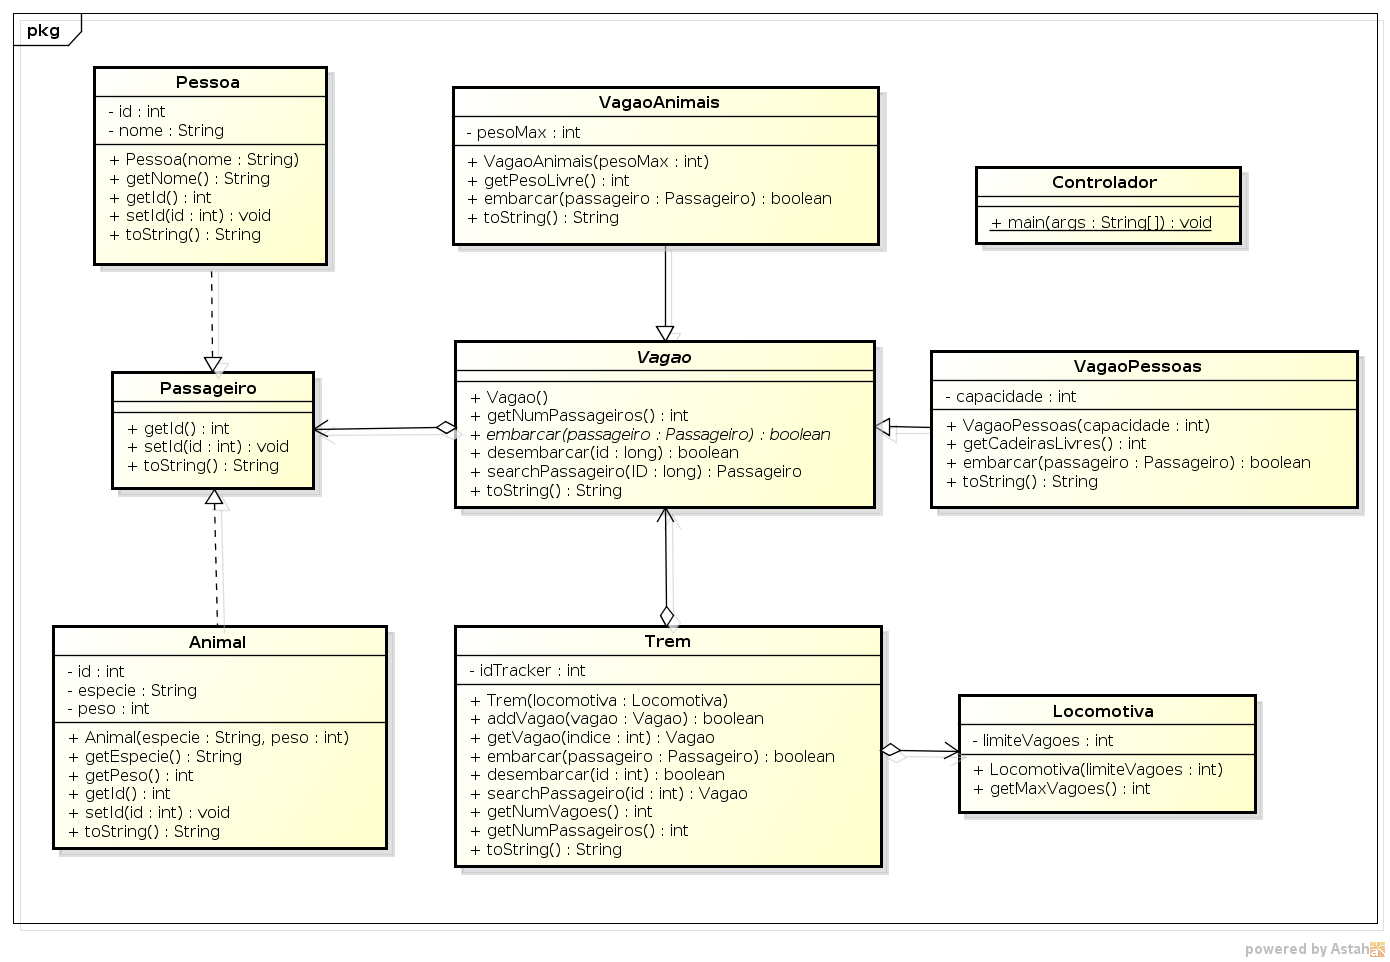
\includegraphics[width=1\linewidth]{./diagrama}
\caption{Diagrama de Classes}
\label{fig:diagrama}
\end{figure}
%\end{sidewaysfigure}
\end{landscape}

\section{Métodos}
A maioria dos métodos, principalmente os \bf{get} e \bf{set} são de implementação trivial. Os métodos não
triviais estão descritos abaixo.

\subsection{Controlador}
O controlador mais uma vez é brinde. Dado, o controlador apresentado na Listings \ref{controlador}, a saída gerada deve ser algo como:

\begin{verbatim}
Trem{
    ( 4:Do )
    [ 1:cao:20 3:gato:10  _:5 ]
    ( 5:Re 6:Mi )
    [ 2:cao:30  _:0 ]
}
\end{verbatim}

\pagebreak
\lstinputlisting[label=controlador, caption=Controlador, float=h]{controlador.java}

\subsection{Trem e Locomotiva}
\begin{itemize}
\item A classe Locomotiva é igual ao volume 1.
\item Na classe Trem o único método alterado é o \tt{toString()}. Ele contrói a String interando sobre os vagões e montando a String usando 

\verb|"\t" + vagao.toString() + "\n"|
\end{itemize}

\subsection{Passageiro}
	\begin{itemize}
		\item O Passageiro se tornou uma interface.
		\item Método \tt{toString()} retorna todos os atributos da classe no formato
		
		\verb|"id:atr1:atr2"|
	\end{itemize}


\subsection{Pessoa}
	\begin{itemize}
	\item Pessoa implementa Passageiro. Possui além do id, uma atributo nome.
	\item O método \tt{String toString()} retorna \verb|"id:nome"|
	\end{itemize}
	
\subsection{Animal}
	\begin{itemize}
	\item Animal implementa Passageiro. Possui além do id, uma atributo espécie e um peso.
	\item O método \tt{String toString()} retorna \verb|"id:especie:peso"|
	\end{itemize}
	
\subsection{Vagao}
\begin{itemize}
\item Vagão se tornou classe abstrata. Perdeu o método
\tt{getCapacidade} e o atributo \tt{capacidade}. A classe \tt{embarcar} tornou-se abstrata.
\item O Vetor de passageiros se tornou \tt{protected} para que possa ser acessado pelas classes derivadas.
\item Método \tt{String toString()} retorna uma String contendo a descrição dos passageiros do vagão. Deve
concatenar as chamadas \tt{toString()} dos passageiros.

\verb|"1:Carlos 2:Mario"|

\end{itemize}

\subsection{VagaoPessoas}
\begin{itemize}
\item VagaoPessoas extende a classe abstrata Vagao. Possui um atributo capacidade que define quantas cadeiras disponíveis existem. 
\item Método \tt{boolean embarcar(Passageiro passageiro)} verifica se existe cadeira vaga, verifica se o passageiro é do tipo pessoa e então adiciona o passageiro. Use \tt{passageiro instanceof Pessoa}.
\item Método \tt{String toString()} inicia e termina com parênteses, chama o método \tt{super.toString()} para
pegar a lista de passageiros e adiciona um \tt{_} para cada cadeira vaga. Um exemplo de saída
para um vagão de capacidade 5, com 2 pessoas seria:

\verb|( 4:Carlos 5:Mario _ _ _ )|
\end{itemize}

\subsection{VagaoAnimais}
\begin{itemize}
\item \tt{VagaoAnimais} extende a classe abstrata \tt{Vagao}. Possui um atributo pesoMax que define qual o peso total que ele comporta. 
\item Método \tt{boolean embarcar(Passageiro passageiro)} verifica se o passageiro é do tipo animal, verifica se o animal ainda cabe e então adiciona o passageiro. Use \tt{passageiro instanceof Animal}.
\item Método \tt{String toString()} inicia e termina com colchetes, chama o método \tt{super.toString()} para
pegar a lista de passageiros e adiciona um \tt{_:pesoLivre} para cada cadeira vaga. Um exemplo de saída para um vagão de capacidade 500, com 3 animais de 100 kilos seria:

\verb|[ 1:Cao:100 2:Gato:100 3:Porco:100 _:200 ]|
\end{itemize}

\end{document}
